\begin{activity}\label{A:0.6.2}
	For each of the following graphs, find a possible formula for the polynomial of lowest degree that fits the graph.
    \def\scl{0.7}
				\begin{center}
%                     \begin{tikzpicture}[scale=\scl]
%                         \begin{axis}[axis lines=center, xmin=-4, xmax=2, ymin=-5, ymax=2,
%                             title={Plot (a)}]
%                             \addplot[very thick, blue, smooth,samples=100,domain=-4.0:2.0] {((x)-1.0)*((x)+3.0)};
%                         \end{axis}
%                     \end{tikzpicture}
%                     \begin{tikzpicture}[scale=\scl]
%                         \begin{axis}[axis lines=center, xmin=-3, xmax=3.5, ymin=-8.5, ymax=6,
%                             title={Plot (b)}, ytick={-8,-6,-4,-2,2,4,6}]
%                             \addplot[very thick, blue, smooth,samples=100,domain=-3:3.5] {0-((x)+2.0)*((x)-3.0)*((x)-1.0)};
%                         \end{axis}
%                     \end{tikzpicture}
%                     \begin{tikzpicture}[scale=\scl]
%                         \begin{axis}[axis lines=center, xmin=-2, xmax=3, ymin=-3, ymax=2,
%                             title={Plot (c)}]
%                             \addplot[very thick, blue, smooth,samples=100,domain=-2:3] {((x)+1.0)*((x)-2.0)*((x)-1.0)*((x)-1.0)};
%                         \end{axis}
%                     \end{tikzpicture}
% % 					\begin{tikzpicture}[line cap=round,line join=round,>=triangle 45, x=1.0cm, y=0.86cm] 
% % 						\draw[->,color=black] (-4.0,0.0) -- (2.0,0.0);
% % 						\foreach \x in {-4,-3,-2,-1,1}
% % 						\draw[shift={(\x,0)},color=black] (0pt,2pt) -- (0pt,-2pt) node[below] {\footnotesize $\x$};
% % 						\draw[->,color=black] (0.0,-5.0) -- (0.0,2.0);
% % 						\foreach \y in {-5,-4,-3,-2,-1,1}
% % 						\draw[shift={(0,\y)},color=black] (2pt,0pt) -- (-2pt,0pt) node[left] {\footnotesize $\y$};
% % 						\draw[color=black] (0pt,-10pt) node[right] {\footnotesize $0$};
% % 						\clip(-4.0,-5.0) rectangle (2.0,2.0);
% % 						\draw[very thick, blue, smooth,samples=100,domain=-4.0:2.0] plot(\x,{((\x)-1.0)*((\x)+3.0)});
% % 					\end{tikzpicture}   
% % 					\begin{tikzpicture}[line cap=round,line join=round,>=triangle 45, x=0.86cm, y=0.33cm] 
% % 						\draw[<->,color=black] (-3.5,0.0) -- (3.5,0.0); 
% % 						\foreach \x in {-3,-2,-1,1,2,3} 
% % 						\draw[shift={(\x,0)},color=black] (0pt,2pt) -- (0pt,-2pt) node[below] {\footnotesize $\x$}; 
% % 						\draw[->,color=black] (0.0,-10) -- (0.0,8); 
% % 						\foreach \y in {-8,-6,-4,-2,2,4,6}
% % 						\draw[shift={(0,\y)},color=black] (2pt,0pt) -- (-2pt,0pt) node[left] {\footnotesize $\y$}; 
% % 						\draw[color=black] (0pt,-10pt) node[right] {\footnotesize $0$}; 
% % 						\clip(-3.5,-10) rectangle (3.5,8); 
% % 						\draw[very thick, blue, smooth,samples=100,domain=-3.5:3.5] plot(\x,{0-((\x)+2.0)*((\x)-3.0)*((\x)-1.0)});
% % 					\end{tikzpicture}   
% % 					\begin{tikzpicture}[line cap=round,line join=round,>=triangle 45, x=1.2cm, y=1.1cm] 
% % 						\draw[<->,color=black] (-2,0.0) -- (3,0.0); 
% % 						\foreach \x in {-2,-1,1,2,3} 
% % 						\draw[shift={(\x,0)},color=black] (0pt,2pt) -- (0pt,-2pt) node[below] {\footnotesize $\x$}; 
% % 						\draw[->,color=black] (0.0,-3.5) -- (0.0,2); 
% % 						\foreach \y in {-3,-2,-1,1,2}
% % 						\draw[shift={(0,\y)},color=black] (2pt,0pt) -- (-2pt,0pt) node[left] {\footnotesize $\y$}; 
% % 						\draw[color=black] (0pt,-10pt) node[right] {\footnotesize $0$}; 
% % 						\clip(-2,-3.5) rectangle (3,2); 
% % 						\draw[very thick, blue, smooth,samples=100,domain=-2:3] plot(\x,{((\x)+1.0)*((\x)-2.0)*((\x)-1.0)*((\x)-1.0)}); 
% % 					\end{tikzpicture}   
                    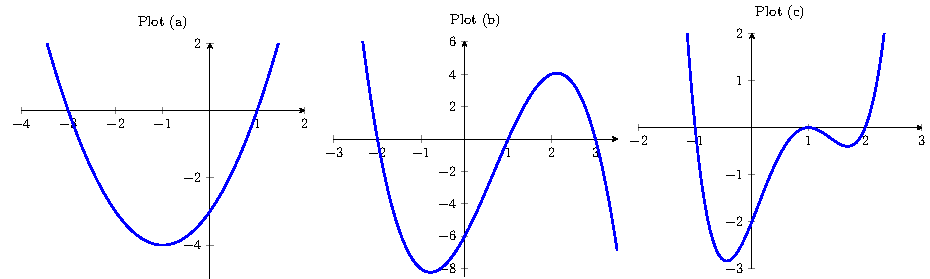
\includegraphics[width=0.99\columnwidth]{figures/0-6-fig5.pdf}
				\end{center}      
\end{activity}
\begin{smallhint}
How many roots are there and how do the ends behave?
\end{smallhint}
\begin{bighint}
    You may want to use Theorems \ref{T:0.6.1} and \ref{T:0.6.2} to determine the degree
    of the polynomial as well as the roots and factors.
\end{bighint}
\begin{activitySolution}
   \ba
        \item This function clearly has two roots and the ends show the same behavior.
            This indicates that this is likely a degree 2 polynomial (a quadratic).  Based
            on the roots $x=-2$ and $x=1$ the factors are $(x+2)$ and $(x-1)$ so the
            polynomial is of the form $a(x) = C(x+2)(x-1)$.  Finally, it appears that the
            point $(-1,-4)$ is on the curve so $C=2$ and the polynomial is 
            \[ a(x) = 2(x+2)(x-1). \]
        \item This function clearly has three roots and the ends show the opposite
            behavior.  Since the right-hand side of the function tends down we expect a
            negative leading coefficient.  Based on the roots $x=-2$, $x=1$, and $x=3$ the
            factors are $(x+2)$, $(x-1)$, and $(x-3)$ and the polynomial takes the form
            $b(x) = C(x+2)(x-1)(x-3)$.  The point $(-1,-8)$ appears to be on the graph so
            $C = -1$ and the polynomial is
            \[ b(x) = -(x+2)(x-1)(x-3). \]
        \item This function clearly has three roots but the end behavior indicates an even
            degree polynomial.  The root at $x=1$ is special since we do not cross the $x$
            axis.  Hence, the factors are $(x+1)$, $(x-1)$, $(x-1)$, and $(x-2)$.  Notice
            that the $(x-1)$ root is listed twice, and hence the polynomial takes the form
            $c(x) = C(x+1)(x-1)^2(x-2)$.  The point $(0,-2)$ appears to be on the graph so
            $C = 1$ and the polynomial is
            \[ c(x) = (x+1)(x-1)^2(x-2). \]
   \ea
\end{activitySolution}

\aftera
